\documentclass{beamer}
\usepackage[utf8]{inputenc}

\usetheme{Madrid}
\usecolortheme{default}
\usepackage{amsmath,amssymb,amsfonts,amsthm}
\usepackage{txfonts}
\usepackage{tkz-euclide}
\usepackage{listings}
\usepackage{adjustbox}
\usepackage{array}
\usepackage{tabularx}
\usepackage{gvv}
\usepackage{lmodern}
\usepackage{circuitikz}
\usepackage{tikz}
\usepackage{graphicx}

\setbeamertemplate{page number in head/foot}[totalframenumber]

\usepackage{tcolorbox}
\tcbuselibrary{minted,breakable,xparse,skins}



\definecolor{bg}{gray}{0.95}
\DeclareTCBListing{mintedbox}{O{}m!O{}}{%
	breakable=true,
	listing engine=minted,
	listing only,
	minted language=#2,
	minted style=default,
	minted options={%
		linenos,
		gobble=0,
		breaklines=true,
		breakafter=,,
		fontsize=\small,
		numbersep=8pt,
		#1},
	boxsep=0pt,
	left skip=0pt,
	right skip=0pt,
	left=25pt,
	right=0pt,
	top=3pt,
	bottom=3pt,
	arc=5pt,
	leftrule=0pt,
	rightrule=0pt,
	bottomrule=2pt,
	toprule=2pt,
	colback=bg,
	colframe=orange!70,
	enhanced,
	overlay={%
		\begin{tcbclipinterior}
			\fill[orange!20!white] (frame.south west) rectangle ([xshift=20pt]frame.north west);
	\end{tcbclipinterior}},
	#3,
}
\lstset{
	language=C,
	basicstyle=\ttfamily\small,
	keywordstyle=\color{blue},
	stringstyle=\color{orange},
	commentstyle=\color{green!60!black},
	numbers=left,
	numberstyle=\tiny\color{gray},
	breaklines=true,
	showstringspaces=false,
}
\begin{document}

\title 
{4.3.30}
\date{12 September,2025}

\author 
{Naman Kumar-EE25BTECH11041}
\graphicspath{./figs}


\frame{\titlepage}
\begin{frame}{Question}
Find the equation of the line which passes through the point $(-4, 3)$ and the portion of the line intercepted between the axes is divided internally in ratio 5:3 by this point.
\end{frame}
\begin{frame}{Solution}
Let the intercept points be
\begin{align}
    \vec{P}=a\vec{e_1},\vec{Q}=b\vec{e_2} \\\vec{e_1}=\begin{pmatrix}1\\0\end{pmatrix}, \vec{e_2}=\begin{pmatrix}0\\1\end{pmatrix}, \text{a and b are constants}
\end{align}
and
\begin{align}
    \vec{R}=\begin{pmatrix}-4\\3\end{pmatrix}=-4e_1+3e_2
\end{align}
be the given point.\\
Using
\begin{align}
    \vec{R}=\frac{k\vec{Q}+\vec{P}}{k+1} \label{section}\\
    \vec{R}=\frac{5\times b\vec{e_2}+3\times a\vec{e_1}}{8}
\end{align}
\end{frame}
\begin{frame}{Solution}
\begin{align}
    -4\vec{e_1}+3\vec{e_2}=\frac{5\times b\vec{e_2}+3\times a\vec{e_1}}{8}\\
    -32\vec{e_1}+24\vec{e_2}=3a\vec{e_1}+5b\vec{e_2} \label{points}
\end{align}
General equation of line
\begin{align}
    \vec{x}=\vec{h}+c\vec{m}
\end{align}
Where\\
\begin{table}[h!]
    \centering
    \begin{tabular}{|c|c|}
        \hline
        Point & Coordinates \\
        \hline
	    $A$ & $\myvec{1\\-1}$ \\
	    $B$ & $\myvec{-4\\2k}$ \\
	    $C$ & $\myvec{-k\\-5}$ \\
        \hline
    \end{tabular}
    \caption{Vertices of $\triangle ABC$ before substituting $k$}
    \label{tab:triangle_k}
\end{table}

\end{frame}
\begin{frame}{Solution}
Slope is
\begin{align}
\vec{m}=\vec{Q}-\vec{P}\\
\end{align}
let $\vec{h}=\vec{P}$\\
So, Equation of line is
\begin{align}
    \vec{x}=\vec{h}+c\vec{m}\\
    \vec{x}=\vec{P}+c(\vec{Q}-\vec{P})
\end{align}
Putting values of $\vec{Q},\vec{P}$
\begin{align}
    \vec{x}=a\vec{e_1}+c(b\vec{e_2}-a\vec{e_1})
\end{align}
\end{frame}
\begin{frame}{Solution}
Comparing terms in \eqref{points} for values of a and b
\begin{align}
    \vec{x}=\frac{-32}{3}\vec{e_1}+c(\frac{24}{5}\vec{e_2}-\frac{-32}{3}\vec{e_1})
\end{align}
Therefore Final equation is
\begin{align}
\begin{pmatrix}x\\y\end{pmatrix}=\begin{pmatrix}\frac{-32}{3}\\0\end{pmatrix}+k\begin{pmatrix}\frac{32}{3}\\ \frac{24}{5}\end{pmatrix}
\end{align}
\end{frame}
\begin{frame}{Figure}
\begin{figure}[H]
    \centering
    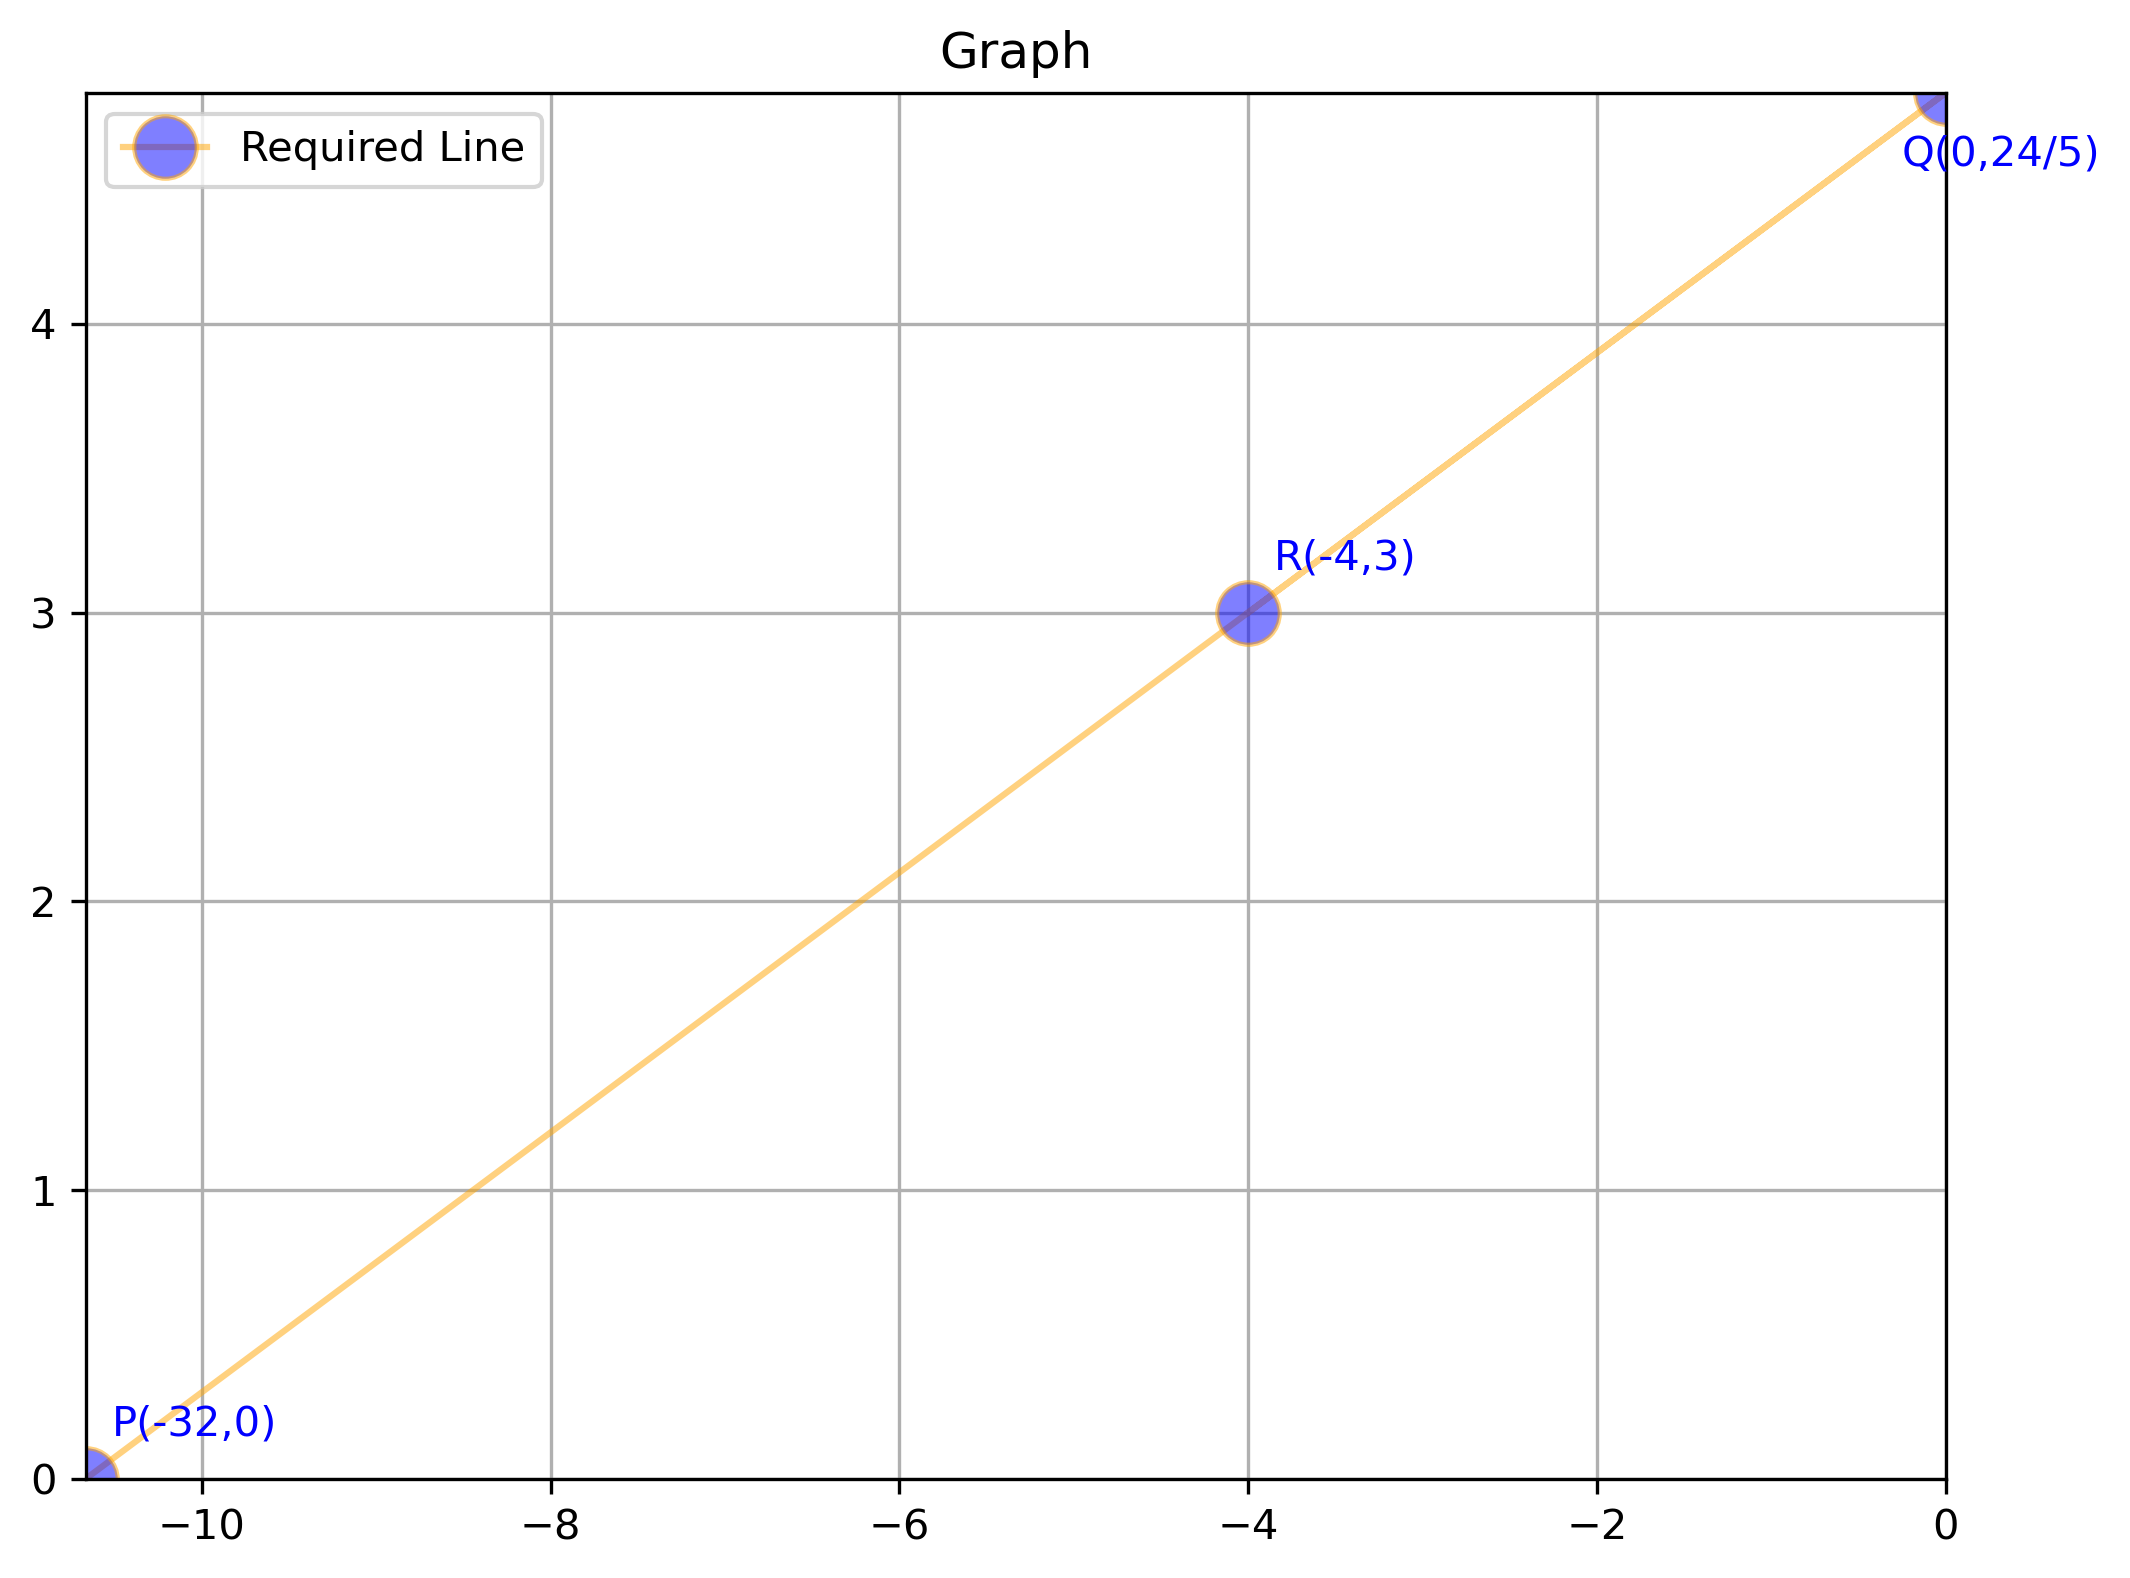
\includegraphics[width=0.9\columnwidth]{figs/figure.png}
    \label{fig:placeholder}
\end{figure}
\end{frame}
\begin{frame}[fragile]
\frametitle{C code}
\begin{lstlisting}
#include <stdio.h>

void trisec(double k, double x1, double y1, double x2, double y2, double* a, double* b){
    *a= (x1+k*x2)/(1+k);
    *b= (y1+k*y2)/(1+k);
}
\end{lstlisting}
\end{frame}
\begin{frame}[fragile]
\frametitle{Python code}
\begin{lstlisting}
import ctypes
import numpy as np
import matplotlib.pyplot as plt

# Load shared object
lib = ctypes.CDLL("./main.so")

# Define function signature
lib.trisec.argtypes = [
    ctypes.c_double,  # k
    ctypes.c_double,  # x1
    ctypes.c_double,  # y1
    ctypes.c_double,  # x2
    ctypes.c_double,  # y2
    ctypes.POINTER(ctypes.c_double),  # *a
    ctypes.POINTER(ctypes.c_double)   # *b
]
\end{lstlisting}
\end{frame}
\begin{frame}[fragile]
\frametitle{Python code}
\begin{lstlisting}
# Known intercepts from math derivation
a = -32.0/3.0
b = 24.0/5.0

# Call trisec with k = 5/3
px = ctypes.c_double()
py = ctypes.c_double()
lib.trisec(5.0/3.0, a, 0.0, 0.0, b, ctypes.byref(px), ctypes.byref(py))

print(f"Computed point dividing AB in 5:3 = ({px.value}, {py.value})")
\end{lstlisting}
\end{frame}
\begin{frame}[fragile]
\frametitle{Python code}
\begin{lstlisting}
# Now plot line
x_vals = np.linspace(a, 0, 200)
y_vals = b*(1 - x_vals/a)

plt.plot(x_vals, y_vals, label="Line through intercepts")
plt.scatter([a,0], [0,b], color="green", label="Intercepts")
plt.scatter([-4], [3], color="red", marker="x", s=100, label="Given point (-4,3)")
plt.axhline(0, color="black", linewidth=0.5)
plt.axvline(0, color="black", linewidth=0.5)
plt.legend()
plt.grid(True)
plt.show()
\end{lstlisting}
\end{frame}
\begin{frame}[fragile]
\frametitle{Direct Python code}
\begin{lstlisting}
import numpy as np
import matplotlib.pyplot as plt

plt.figure(figsize=(8, 6), dpi=100)

x = np.array([-32/3, 0, -4])
y= np.array([0, 24/5, 3])
plt.plot(x,y,'o-', color='orange',mfc='blue',ms='15',alpha=0.5, label="Required Line")
\end{lstlisting}
\end{frame}
\begin{frame}[fragile]
\frametitle{Direct Python code}
\begin{lstlisting}
plt.text(x[0]+0.15, y[0]+0.15, "P(-32,0)", color='blue')
plt.text(x[1]-0.25, y[1]-0.25, "Q(0,24/5)", color='blue')
plt.text(x[2]+0.15, y[2]+0.15, "R(-4,3)", color='blue')
plt.legend()
plt.title("Graph")
plt.grid()
plt.xlim(-32/3, 0)
plt.ylim(0, 24/5)

plt.savefig('figure.png', dpi=300, bbox_inches='tight')
plt.show()
\end{lstlisting}
\end{frame}

\end{document}